\chapter{Fusões de Lógicas Modais}
    \label{cap:FusoesLogicasModais}
    A fusão de lógicas modais é o método mais simples de combinar duas lógicas modais, segundo~\citeshort{gabbay2003many}. Combinações de lógicas
    é um tópico relativamente recente no estudo da lógica moderna, de acordo com~\citeshort{sep-logic-combining}. Consiste de métodos para sintetizar
    novos sistemas lógicos a partir de sistemas já existentes, seja por meio da junção de diversos sistemas em um único ou pela separação de um sistema
    lógico em diversos sistemas componentes~\cite{carnielli2008analysis}. A ideia fundamental por trás da combinação de lógicas é que sistemas lógicos
    podem ser ``reutilizados'', gerando sistemas mais expressivos mas que possuam as mesmas propriedades úteis dos sistemas lógicos base~\cite{roggia2012fusion}.

    A combinação de lógicas é uma ferramenta para tratar problemas tanto práticos quanto filosóficos. Por exemplo, linguagens lógicas que tratam de espaço,
    tempo e conhecimento podem ser combinadas num sistema lógico ideal para raciocinar sobre sistemas multiagentes. Já linguagens lógicas que tratam de
    obrigatoriedade e possibilidade podem ser combinadas para tratar do problema da ``Obrigação implica Possibilidade'', onde o fato que algo é obrigatório
    implica que é logicamente possível de ser feito ou ocorrer~\cite{carnielli2008analysis}.

    Segundo~\citeshort{carnielli2008analysis}, a fusão de lógicas modais pode ser vista como um mecanismo de combinação de lógicas \(\odot\), tal que, dadas duas
    lógicas \Mathcali{L}{1} e \Mathcali{L}{2}, gera uma nova lógica \(\mathcal{L}_{12} = \mathcal{L}_1 \Odot \mathcal{L}_2\). A lógica \Mathcali{L}{12}
    é então definida como uma extensão (máxima ou mínima) das lógicas base, isto é, estende a linguagem, semântica e sintaxe de \Mathcali{L}{1} e \Mathcali{L}{2}
    de maneira controlada, de forma que nenhuma característica indesejada seja inclusa em \Mathcali{L}{12}. Mais ainda, as lógicas base devem ser apresentadas da mesma
    forma, por exemplo, duas lógicas modais apresentadas semanticamente por uma semântica de mundos possíveis e sintaticamente por uma axiomatização de Hilbert.

    O estudo de combinações de lógicas modais se iniciou, segundo~\citeshort{roggia2012fusion}, com~\citeshort{fitting1969logics}, onde o autor apresenta sistemas lógicos
    resultantes de combinações de S4, S5 e sistemas lógicos deônticos por um método semelhante à fusão, já~\citeshort{thomason1984combinations} introduziu
    o termo ``fusão'' e definiu sistematicamente a fusão de lógicas modais. Ademais, segundo~\citeshort{sep-logic-combining}, a fusão definida por
    \citeauthoronline{thomason1984combinations} foi o primeiro método genérico de combinações de lógicas.

    No que segue, será apresentada a fusão de lógicas modais e suas propriedades de acordo com a formulação de \citeshort{gabbay2003many}.
    \begin{definicao}[Fusão de Lógicas Modais]
        \label{def:Fusao}
        Sendo \Mathcali{L}{1} e \Mathcali{L}{2} lógicas monomodais, cujas linguagens \(\mathsf{LM}_1\) e \(\mathsf{LM}_2\) são definidas sobre as assinaturas
        \(\mathsf{C}_{1}\) e \(\mathsf{C}_{2}\) com modalidades \BOXi{1} e \BOXi{2} distintas entre si\footnote{Isto é, \BOXi{1} e \BOXi{2} são interpretadas de maneira diferente.},
        correspondentes às classes de frames \Mathfraki{F}{1} e \Mathfraki{F}{2}, sendo \(\langle \mathcal{W}, \mathcal{R}\rangle\) e \(\langle \mathcal{W}, \mathcal{S}\rangle\)
        seus respectivos representantes\footnote{Note que o conjunto de mundos \Mathcal{W} é o mesmo em todos os frames de ambas as classes.}, e
        axiomatizadas por \(\langle\Lambda_{\mathsf{LM}_1} \Oplus \Xi_1, \{\funcao{Nec}_{1}, \funcao{MP}\}\rangle\) e
        \(\langle\Lambda_{\mathsf{LM}_2} \Oplus \Xi_2, \{\funcao{Nec}_2, \funcao{MP}\}\rangle\).

        A lógica \(\mathcal{L}_{12} = \mathcal{L}_1 \Odot \mathcal{L}_2\) resultante da fusão de \Mathcali{L}{1} com \Mathcali{L}{2} terá linguagem
        \(\mathsf{LM}_{12}\) definida sobre a assinatura \(\mathsf{C}_{12} = \mathsf{C}_1 \cup \mathsf{C}_2\), será correspondente à classe \Mathfraki{F}{12}
        de 2-frames da forma \(\langle \mathcal{W}, \mathcal{R}, \mathcal{S}\rangle\) e será axiomatizada por
        \(\langle\Lambda_{\mathsf{LM}_{12}} \Oplus (\Xi_1 \Oplus \Xi_2), \{\funcao{Nec}_1, \funcao{Nec}_2, \funcao{MP}\}\rangle\). \qed
    \end{definicao}

    Como \(\mathsf{LM}_1\) e \(\mathsf{LM}_2\) não compartilham modalidades, \Mathcali{L}{12} será dita \textit{independentemente axiomatizável} como apresentado
    por~\citeshort{kracht1991properties}. A operação de fusão é associativa e comutativa~\cite{gabbay2003many}, e a fusão de lógicas modais
    pode ser vista como uma forma de obter as lógicas multimodais descritas na Seção~\ref{sec:LM-Multimodais}. O caso de fusões de lógicas multimodais
    é uma generalização do caso acima, onde \(\mathsf{LM}_1\) e \(\mathsf{LM}_2\) são linguagens multimodais e os demais conceitos são generalizados de acordo.

    \begin{exemplo}[Lógica Epistêmica como Fusão]
        Como apresentado em~\citeshort{gabbay2003many}, considerar lógicas epistêmicas como fusões de lógicas aléticas é algo simples. Considere
        \Mathcali{L}{A}, \Mathcali{L}{B} e \Mathcali{L}{C} lógicas monomodais aléticas cujas modalidades representam o conhecimento de agentes
        A, B e C respectivamente. Caso seja desejado um sistema lógico que modele interação entre os agentes, é necessário descrever um
        formalismo que seja capaz de expressar tanto o conhecimento de cada agente sobre o mundo ao seu redor, quanto o conhecimento de cada
        agente sobre o conhecimento \textit{dos outros} agentes. Esse sistema é obtido pela fusão das lógicas \Mathcali{L}{A}, \Mathcali{L}{B}
        e \Mathcali{L}{C} em um único sistema lógico \Mathcali{L}{ABC}. Os axiomas deste sistema que contém alguma modalidade descrevem o
        conhecimento do seu respectivo agente, mas, por definição, todos os axiomas contém apenas uma modalidade, logo não há nenhum
        axioma que explicitamente relaciona o conhecimento de dois agentes distintos.

        Porém, não é difícil imaginar situações onde interações entre os agente são necessárias, por exemplo caso um agente saiba tudo o que o
        outro sabe. Para lidar com essas restrições, basta adicionar novos axiomas na axiomatização de \Mathcali{L}{ABC}. Por exemplo,
        caso seja necessário representar a afirmação ``o agente \textit{A} sabe tudo o que o agente \textit{B} sabe'' basta adicionar o axioma
        \(\Box_B p_0 \to \Box_A p_0\) na axiomatização de \Mathcali{L}{ABC}\footnote{Obtendo então um sistema \(\mathcal{L}_{ABC}'\).}.\qed
    \end{exemplo}

    Este capítulo é organizado da seguinte forma: na Seção~\ref{sec:Preservacao} será apresentado o conceito de preservação de propriedades pela fusão de lógicas modais
    e será provada a transferência de algumas propriedades pela fusão e na Seção~\ref{sec:SistemaKT4} será apresentado o sistema bimodal \SisT, que será utilizado
    posteriormente para a prova de conceito de fusão de lógicas modais em Coq.

    \section{Preservação de Propriedades}
        \label{sec:Preservacao}
        Uma das mais importantes características da fusão de lógicas modais é a preservação de propriedades, também chamada de transferência de teoremas
        por~\cite{fine1996transfer}. Segundo \cite{kracht1991properties}, uma propriedade é dita preservada pela fusão se, sendo \Mathcali{L}{12}
        uma lógica multimodal resultante da fusão de duas lógicas (multi)modais \Mathcali{L}{1} e \Mathcali{L}{2}, caso \Mathcali{L}{1} e \Mathcali{L}{2}
        satisfaçam alguma propriedade \textit{P}, então \Mathcali{L}{12} também ira satisfazer \textit{P}.

        Dentre as propriedades que são preservadas pela fusão de lógicas modais, têm-se as descritas na Seção~\ref{sec:LM-MetaPropriedades}.
        No restante da seção, serão apresentados conceitos e provas referentes à preservação das propriedades de corretude e completude, retirados de~\citeshort{fine1996transfer}.

        Em~\citeshort{fine1996transfer}, os autores consideram uma lógica monomodal como um conjunto de fórmulas, como foi descrito na Seção~\ref{sec:LM-LogicaComoConjunto}.
        Para manter consistência com a prova original, usaremos esta definição de lógica pelo restante da seção.
        Conceitos semânticos, como frames, modelos e classes destes não são alterados.

        \begin{definicao}[Fusão de Lógicas como Conjuntos]
            \label{def:FusaoLogicasConjunto}
            Sendo \Mathcali{L}{1} e \Mathcali{L}{2} lógicas monomodais cujas linguagens são \linguagem{1} e \linguagem{2} e são definidas com base nos conjuntos
            \(\Lambda_{\mathsf{LM}_{1}}\) e \(\Lambda_{\mathsf{LM}_{2}}\). A lógica \Mathcali{L}{12} resultante da fusão de \Mathcali{L}{1} e \Mathcali{L}{2} terá
            linguagem \linguagem{12} (obtida da forma descrita na Definição~\ref{def:Fusao}) e será definida (remeta à Definição~\ref{def:LogicaConjunto})
            com base no conjunto \(\Lambda_{\mathsf{LM}_{1}} \mathbin{\cup} \Lambda_{\mathsf{LM}_{2}}\).
        \end{definicao}

        \begin{definicao}[Frames e Modelos para Lógicas]
            Sendo \Mathcal{L} uma lógica, um frame (modelo) \Mathcal{S} é dito um frame (modelo) \textit{para \Mathcal{L} se, e somente se, \Mathcal{L} é válida em
            \Mathcal{S}}\footnote{Veja as definições~\ref{def:ValidadeModelo} e~\ref{def:ValidadeFrame}.}. \qed
        \end{definicao}

        No restante desta sessão, serão analisadas duas lógicas monomodais \Mathcali{L}{1} e \Mathcali{L}{2} cujas linguagens são \(\mathsf{LM}_1\) e \(\mathsf{LM}_2\),
        estas são combinadas numa lógica bimodal \Mathcali{L}{12} cuja linguagem é \(\mathsf{LM}_{12}\). As linguagens \(\mathsf{LM}_{1}, \mathsf{LM}_{2} \text{ e } \mathsf{LM}_{12}\)
        são definidas de forma análoga à linguagem \textsf{LM} apresentada na Definição~\ref{def:LinguagemModal}, porém são baseadas nas assinaturas minímas
        \(\mathsf{C}_1 = \{\lor, \neg, \Box_{1}\}\), \(\mathsf{C}_2 =\{\lor, \neg, \Box_{2}\}\) e \(\mathsf{C}_{12} = \{\lor, \neg, \Box_{1}, \Box_{2}\}\)
        respectivamente. Os conectivos \(\land, \to, \Diamond_1 \text{ e } \Diamond_2\) são abreviações definidas a partir das dualidades apresentadas na Definição~\ref{def:Dualidade}.

        % Sendo \SIGMA o conjunto contendo todas as tautologias proposicionais, o axioma \(K_1\) e o axioma \(K_2\), \Mathcali{L}{12} é exatamente o conjunto definido pelo fecho de
        % \SIGMA para as operações de Substituição (Definição~\ref{def:Substituicao}), Modus Ponens (Definição~\ref{def:RegrasInferencia}), Necessitação para \BOXi{1} e
        % Necessitação para \BOXi{2} (Definição~\ref{def:AxiomatizacaoMultimodal}).

        Denotaremos por \Mathfraki{F}{1} e \Mathfraki{F}{2} as classes de frames de \Mathcali{L}{1} e \Mathcali{L}{2} e denotaremos por
        \(\mathfrak{F}_{12} = \mathfrak{F}_1 \Otimes \mathfrak{F}_2\) a classe de 2-frames \(\{\langle \mathcal{W}, \mathcal{R}_1, \mathcal{R}_2 \rangle \ | \
        \langle \mathcal{W}, \mathcal{R}_1 \rangle \in \mathfrak{F}_1 \text{ e } \langle \mathcal{W}, \mathcal{R}_2 \rangle \in \mathfrak{F}_2\}\),
        da lógica \Mathcali{L}{12}. Análogo para modelos e classes de modelos.

        \subsection{Preservação de Corretude}
            \label{subsec:PreservacaoCorretude}
            % Antes de provar que a corretude é preservada pela fusão, devemos apresentar o conceito de corretude novamente, devido a interpretação
            % diferente do conceito de lógica. Note que a definição de corretude a seguir é análoga à Definição~\ref{def:Corretude}.

            % \begin{definicao}[Corretude]
            %     Uma lógica \Mathcal{L} é dita \textit{correta com relação a uma classe de frames \Mathfrak{F}} se, e somente se, se \(\phi \in \mathcal{L}\) então
            %     \(\mathfrak{F} \vDash \phi\). \qed
            % \end{definicao}

            % Note que, afirmar que uma classe de frames \Mathfrak{F} é uma classe de frames para alguma lógica \Mathcal{L} é o mesmo que afirmar que \Mathcal{L}
            % é correta com relação à \Mathfrak{F}.

            Considerando a Definição~\ref{def:CorretudeConjunto} que apresenta o conceito de completude para lógicas descritas como conjuntos, temos o seguinte
            teorema:

            \begin{teorema}[Transferência de Corretude]
                \label{teo:TransCorretude}
                Sendo \Mathcali{L}{1} e \Mathcali{L}{2} lógicas modais corretas com relação às classes de frames \Mathfraki{F}{1} e \Mathfraki{F}{2},
                \(\mathcal{L}_{12} = \mathcal{L}_{1} \Odot \mathcal{L}_{2}\) será correta com relação a classe de frames \(\mathfrak{F}_{12} = \mathfrak{F}_1 \Otimes \mathfrak{F}_2\).
            \end{teorema}

            \begin{proof}[Prova do Teorema~\ref{teo:TransCorretude}]
                A prova decorre diretamente da definição de \Mathfraki{F}{12} e da corretude de \Mathcali{L}{1} e \Mathcali{L}{2}.
                Como \(\mathfrak{F}_{12} \text{ é uma classe de frames forma } \{ \langle \mathcal{W}, \mathcal{R}_1, \mathcal{R}_2 \rangle \ | \ \langle \mathcal{W}, \mathcal{R}_1 \rangle
                \in \mathfrak{F}_1 \text{ e } \langle \mathcal{W}, \mathcal{R}_2 \rangle \in \mathfrak{F}_2\}\) e ambas as lógicas são corretas, sabemos que todos
                os axiomas proposicionais (Definição~\ref{def:AxiomaisModais}) são válidos em todos os mundos \(w \in \mathcal{W}\) de todo frame
                \(\mathcal{F}_{x} \in \mathfrak{F}_{x}, x \in \{1,2\}\), mais ainda, temos que a regra de Modus Ponens (Definição~\ref{def:RegrasInferencia}) e a
                propriedade de Substituição (Definição~\ref{def:Substituicao}) preservam validade.

                Como \Mathcali{L}{1} é correta para \Mathfraki{F}{1}, sabemos que toda instância de K\textsubscript{1} é válida em todos os mundos \(w \in \mathcal{W}\)
                de todo frame \(\mathcal{F}_{1} \in \mathfrak{F}_{1}\) e que a regra de Necessitação para \BOXi{1} (Definição~\ref{def:AxiomatizacaoMultimodal}) preserva validade.

                Como \Mathcali{L}{2} é correta para \Mathfraki{F}{2}, sabemos que toda instância de K\textsubscript{2} é válida em todos os mundos \(w \in \mathcal{W}\)
                de todo frame \(\mathcal{F}_{2} \in \mathfrak{F}_{2}\) e que a regra de Necessitação para \BOXi{2} (Definição~\ref{def:AxiomatizacaoMultimodal}) preserva validade.
            \end{proof}

        \subsection{Preservação de Completude}
            \label{subsec:PreservacaoCompletude}
            % Antes de apresentar a prova de transferência de completude, devemos apresentar o conceito de consistência com respeito a um conjunto, retirados de~\cite{blackburn2001modal}.
            % % No que segue, usaremos a notação \(\vdash_{\mathcal{L}} \phi\) para indicar que \(\phi \in \mathcal{L}\), e \(\nvdash_{\mathcal{L}} \phi\) para indicar que
            % % \(\phi \notin \mathcal{L}\).

            % % \begin{definicao}[Dedutibilidade]
            % %     Sendo \GAMMA um conjunto de fórmulas, \PHI uma fórmula e \Mathcal{L} uma lógica, é dito que \textit{\PHI é dedutível em \Mathcal{L} a partir de \GAMMA} se
            % %     \(\vdash_{\mathcal{L}} \phi\), ou existem fórmulas \(\gamma_0, \dots, \gamma_n \in \Gamma\) tal que:
            % %     \[
            % %         \vdash_{\mathcal{L}} (\gamma_0 \land \dots \land \gamma_n) \to \phi
            % %     \]
            % %     Caso \PHI seja dedutível em \Mathcal{L} a partir de \GAMMA, escrevemos \(\Gamma \vdash_{\mathcal{L}} \phi\), caso não seja, escrevemos
            % %     \(\Gamma \nvdash_{\mathcal{L}} \phi\). Podemos omitir o subscrito \Mathcal{L} caso não seja necessário explicitar a lógica. \qed
            % % \end{definicao}

            % \begin{definicao}[Consistência com Respeito a Conjunto]
            %     Sendo \GAMMA e \DDELTA conjuntos de fórmulas, \textit{\GAMMA é dito consistente com respeito a \DDELTA, ou \DDELTA-consistente}, se, e somente se,
            %     não existe \(\gamma\) tal que \(\gamma \in \Gamma \text{ e }\neg \gamma \in \Delta\).
            %     Uma \textit{fórmula \PHI é dita \DDELTA-consistente} se \(\{\phi\}\) é \DDELTA-consistente. \qed
            % \end{definicao}

            % Na definição anterior, caso \DDELTA seja uma lógica, \GAMMA será dito consistente com respeito a \DDELTA se \(\Gamma \nvdash_{\Delta} \bot\), pois
            % \(\Gamma \vdash_{\Delta} \bot\) implica que existem fórmulas \(\gamma_0, \dots, \gamma_n \in \Gamma\) tal que
            % \(\vdash_{\Delta} (\gamma_0 \land \dots \land \gamma_n) \to \bot\), ou seja, \(\vdash_{\Delta} \neg (\gamma_0 \land \dots \land \gamma_n) \lor \bot\).
            % Isto é, existe pelo menos um \(\gamma_i\) que pertence à \GAMMA mas não pertence à \DDELTA ou \(\bot \in \Delta\).
            % Caso \(\bot \in \Delta\), \DDELTA é dita uma lógica inconsistente e todo conjunto é inconsistente com respeito à \DDELTA.

            % Com essa definição, podemos então provar o seguinte resultado auxiliar, retirado de~\cite{blackburn2001modal}.

            % \begin{proposicao}
            %     % \label{prop:CompletudeAlternativa}
            %     Uma lógica \Mathcal{L} é dita \textit{fortemente completa para uma classe de frames \Mathfrak{F}}, se, e somente se, todo conjunto de fórmulas
            %     \Mathcal{L}-consistente é satisfazível em algum frame de \Mathfrak{F}.
            %     Uma lógica \Mathcal{L} é dita \textit{fracamente completa para uma classe de frames \Mathfrak{F}}, se, e somente se, toda fórmula
            %     \Mathcal{L}-consistente é satisfazível em algum frame de \Mathfrak{F}.
            % \end{proposicao}

            % Satisfazibilidade em um frame pode ser entendida como satisfazibilidade em qualquer modelo construído com aquele frame. Analogamente para classes de frames.
            % % Na prova abaixo, usamos a notação \(\mathfrak{F}, \Phi \vDash \psi\) para denotar que \PSI é consequência semântica do conjunto \(\Phi\) em algum modelo
            % % construído com algum frame da classe \Mathfrak{F}.

            % \begin{proof}[Prova da Proposição~\ref{prop:CompletudeAlternativa}]
            %     A prova para completude fraca é um caso particular para o caso da completude forte, onde \(\Gamma = \emptyset\), logo, provaremos apenas o caso
            %     da completude forte. A prova é dividida em dois casos; no primeiro caso é provado que se uma lógica é fortemente completa
            %     então todo conjunto consistente é satisfazível, já no segundo caso é provado que se todo conjunto consistente é satisfazível então uma lógica
            %     é fortemente completa. Ambos os casos serão provados por contraposição.

            %     \begin{description}
            %         \item[Caso 1] Supondo algum conjunto de fórmulas \GAMMA e alguma fórmula \PHI tal que \(\Gamma \cup \{\phi\}\) é
            %         \Mathcal{L}-consistente e insatisfazível em \Mathfrak{F}.
            %         Como \(\Gamma \cup \{\phi\}\) é insatisfazível, temos, pela definição de \(\vDash\), que \(\Gamma \cup \{\phi\} \vDash_{\mathcal{M}} \bot\)\footnote{A definição de \(\vDash\)
            %         nos diz que ``Caso o antecedente é satisfazível em todos os mundos de algum modelo \Mathcal{M}, então o consequente também será'' Como \(\Gamma \cup \{\phi\}\) é insatisfazível em
            %         todos os mundos de qualquer modelo \Mathcal{M} construído com qualquer frame da classe \Mathfrak{F}, temos que qualquer fórmula é consequência semântica de \(\Gamma \cup \{\phi\}\).},
            %         em algum modelo \(\mathcal{M} = \langle \mathcal{F}, \mathcal{V} \rangle\) onde \(\mathcal{F} \in \mathfrak{F}\).
            %         Como \(\Gamma \cup \{\phi\}\) é \Mathcal{L}-consistente, temos que \(\Gamma \cup \{\phi\} \nvdash_{\mathcal{L}} \bot\).
            %         Portanto, \Mathcal{L} não é fortemente completo para \Mathfrak{F}.

            %         \item[Caso 2] Supondo que \Mathcal{L} não é fortemente completa com relação à \Mathfrak{F}. Logo, existe um conjunto
            %         de fórmulas \GAMMA e uma fórmula \PHI tal que \(\Gamma \vDash_{\mathfrak{F}} \phi\), porém \(\Gamma \nvdash_{\mathcal{L}} \phi\).
            %         Logo, o conjunto \(\Gamma \cup \{\neg \phi\}\) é \Mathcal{L}-consistente, porém não é satisfazível em qualquer frame da classe \Mathfrak{F}.\qedhere
            %     \end{description}
            % \end{proof}

            % Note que a Proposição~\ref*{prop:CompletudeAlternativa} indica que há uma correspondência entre o conceito de completude com alguma classe de frames
            % e satisfazibilidade de conjuntos \Mathcal{L}-consistente nesta classe.

            Uma lógica é dita (forte ou fracamente) completa se ela é (forte ou fracamente) completa para alguma classe de frames. Ademais, toda lógica é (forte ou fracamente)
            completa para a sua classe de frames correspondentes\footnote{Alternativamente, uma lógica pode ser dita correspondente à alguma classe de frames sse ela
            for (forte ou fracamente) completa para essa classe.}. Logo, para provar que a lógica \(\mathcal{L}_{12} = \mathcal{L}_{1} \Odot \mathcal{L}_{2}\) é completa,
            dada a completude de \Mathcali{L}{1} para \Mathfraki{F}{1} e \Mathcali{L}{2} para \Mathfraki{F}{2}, basta provar que ela é completa para a classe
            \(\mathfrak{F}_{12} = \mathfrak{F}_1 \Otimes \mathfrak{F}_2\) de frames.

            Para demonstrar a preservação de completude, devemos antes apresentar alguns conceitos que são necessários para construir a prova.

            Toda fórmula da linguagem bimodal \(\mathsf{LM}_{12}\) pode ser vista como uma fórmula da linguagem \(\mathsf{LM}_1\) (\(\mathsf{LM}_2\))
            se tratarmos todas as subfórmulas cujo conectivo mais externo é \BOXi{2}(\BOXi{1}) como átomos. Por exemplo, a fórmula:
            \[
                \Box_1 (p_0 \lor p_1) \to \Box_2 (p_3 \land (\Box_1 p_0 \lor \Box_2 p_1))
            \]
            pode ser vista uma fórmula de \(\mathsf{LM}_1\), se tomarmos \(\Box_2 (p_3 \land (\Box_1 p_0 \lor \Box_2 p_1))\) como um átomo:
            \[
                \Box_1 (p_0 \lor p_1) \to \textit{\textbf{p}}_{\left(\Box_2 (p_3 \land (\Box_1 p_0 \lor \Box_2 p_1))\right)}
            \]
            ou como uma fórmula de \(\mathsf{LM}_2\), se tomarmos \(\Box_1(p_0 \lor p_1)\) e \(\Box_1 p_0\) como átomos:
            \[
                \textit{\textbf{p}}_{\left(\Box_1 (p_0 \lor p_1)\right)} \to \Box_2 (p_3 \land (\textit{\textbf{p}}_{\left(\Box_1 p_0\right)} \lor \Box_2 p_1))
            \]

            Usaremos a variável \(\pi \in \{1,2\}\) no lugar dos índices 1 e 2 para indicar uma lógica monomodal e seus componentes (fórmula, frame, modelo, etc.)
            e usaremos a variável \OPI para indicar a lógica monomodal oposta e seus componentes, isto é, \(\pi = 1 \text{ sse } \overline{\pi} = 2\) e vice versa.
            Note que \PI e \OPI são símbolos da nossa metalinguagem e não fazem parte da linguagem da lógica modal, apenas indicam o índice de um objeto qualquer.

            \begin{definicao}[Fragmentos Monomodais e Elementos]
                \label{def:FragmentosMonomodais}
                Sendo \({\boxdot_{\pi} = \{\Box_{\pi} \phi \ | \ \phi \in \mathsf{LM} \}}\) o conjunto de todas as fórmulas cujo conectivo principal é a modalidade \BOXi{\pi},
                podemos definir os \textit{fragmentos \PI-modais de \(\mathsf{LM}_{12}\)} como sendo os menores conjuntos \(\mathsf{LM}_\pi\) que satisfazem as seguintes regras:
                \begin{enumerate}[label=]%[label=\textnormal{\ref{def:FragmentosMonomodais}.\arabic*}]
                    \item \(\mathbb{P} \cup \boxdot_{\overline{\pi}} \subseteq \mathsf{LM}_\pi\)
                    \item \(\text{Se } \phi \in \mathsf{LM}_\pi \text{, então } \circ \phi \in \mathsf{LM}_\pi, \text{ sendo } \circ \in \{\Box_\pi, \neg\}\)
                    \item \(\text{Se } \phi, \psi \in \mathsf{LM}_\pi \text{, então } \phi \lor \psi \in \mathsf{LM}_\pi\)
                \end{enumerate}
                O conjunto \(\Upsilon_\pi = \mathbb{P} \cup \boxdot_{\overline{\pi}}\) é chamado de conjunto de \PI-átomos de uma linguagem
                \(\mathsf{LM}_\pi\)\footnote{Podemos entender \(\Upsilon_\pi\) como as fórmulas que são interpretadas como atômicas em \Mathcali{L}{\pi}.}.
                O conjunto \({\Upsilon = \Upsilon_1 \cup \Upsilon_2}\) é o conjunto de todos os elementos de \(\mathsf{LM}_{12}\), isto é, o conjunto de todas as fórmulas atômicas
                ou cujo conectivo mais externo é uma modalidade. \qed
            \end{definicao}

            \begin{definicao}[\PI-Lógicas, \PIFRAMES e \PIMODELOS]
                Uma \textit{\PI-lógica} é um conjunto \Mathcali{L}{\pi} definido como o fecho do conjunto contendo todos as tautologias e o axioma \textit{K}\textsubscript{\PI}
                para Modus Ponens Necessitação para \BOXi{\pi} e Substituição de fórmulas por elementos de \(\Upsilon_\pi\)\footnote{Análogo à
                Definição~\ref{def:Substituicao}.}\footnote{Essa definição de lógicas pode ser entendida como uma versão mais restrita da definição de lógicas apresentada na
                Definição~\ref{def:LogicaConjunto}.}.

                Um \textit{\PIframe} é um par da forma \(\langle \mathcal{W}, \mathcal{R}_\pi \rangle\) e um \textit{\PImodelo} é uma tripla da forma
                \(\langle \mathcal{W}, \mathcal{R}_\pi, \mathcal{V}_\pi \rangle\) onde \(\mathcal{V}_\pi: \Upsilon_\pi \to 2^{\mathcal{W}}\). \qed
            \end{definicao}

            É importante ressaltar que átomos em \PI-lógicas são termos em \Mathbb{P} e fórmulas cujo conectivo principal é \BOXi{\mOPI}, ou seja, fórmulas cujo
            conectivo principal é \BOXi{\mOPI} são \textit{interpretadas} como átomos na lógica \Mathcali{L}{\pi}.

            \begin{definicao}[\PI-Subfórmulas]
                O conjunto de \textit{\PI-subfórmulas} de uma fórmula \(\phi \in \mathsf{LM}_\pi\), denotado por \(\funcao{Sub}_\pi(\phi)\), é definido indutivamente como
                o menor conjunto que satisfaz as seguintes restrições:
                \begin{align*}
                    &\funcao{Sub}_\pi(p_j)            = \{p_j\}, p_j \in \Upsilon_{\pi} \\
                    &\funcao{Sub}_\pi(\circ \phi)     = \{\circ \phi\} \cup \funcao{Sub}_\pi(\phi), \text{ sendo } \circ \in \{\Box_\pi, \neg\} \\
                    &\funcao{Sub}_\pi(\phi \lor \psi) = \{\phi \lor \psi\} \cup \funcao{Sub}_\pi(\phi) \cup \funcao{Sub}_\pi(\psi) \tag*\qed
                \end{align*}

            \end{definicao}

            No que segue, serão apresentadas diversas funções que operam sobre fórmulas e que são necessárias para a prova de transferência.

            \begin{definicao}[Funções sobre Fórmulas]
                \label{def:FuncoesElementos}
                O conjunto de \textit{\PI-átomos} de uma fórmula \(\phi \in \mathsf{LM}_\pi\), denotado por \(\funcao{C}_\pi(\phi)\), é o conjunto de todas as \PI-subfórmulas de
                \PHI que são interpretadas como atômicas em \linguagem{\pi}. É definido como:
                \[
                    \funcao{C}_\pi(\phi) = \funcao{Sub}_\pi(\phi) \cap \Upsilon_\pi = \{\psi \ | \ \psi \in \funcao{Sub}_{\pi}(\phi) \text{ e }
                        \psi \in (\mathbb{P} \cup \boxdot_{\overline{\pi}})\}
                \]

                O conjunto de \textit{sub-elementos} de uma fórmula \(\phi \in \mathsf{LM}_{12}\), denotado por \(\funcao{SC}(\phi)\), é o conjunto de todas as subfórmulas de \PHI
                que são interpretadas como átomos, isto é, é o \textit{conjunto de todas as subfórmulas de \PHI que são interpretadas como atômicas em \linguagem{\pi} ou
                \linguagem{\mOPI}}. É definido como:
                \[
                    \funcao{SC}(\phi) = \funcao{Sub}(\phi) \cap \Upsilon = \{\psi \ | \ \psi \in \funcao{Sub}(\phi) \text{ e } \psi \in (\mathbb{P} \cup \boxdot_{1} \cup \boxdot_{2})\}
                \]

                O conjunto de \textit{\PI-sub-elementos} de uma fórmula \(\phi \in \mathsf{LM}_\pi\), denotado por \(\funcao{S}_\pi(\phi)\), é o conjunto de todos os sub-elementos de
                \PI-átomos de \PHI, isto é, \textit{é o conjunto de todas as subfórmulas interpretadas como atômicas das \PI-subfórmulas interpretadas como atômicas
                em \(\mathsf{LM}_\pi\) de \PHI}. É definido como:
                \begin{align*}
                    \funcao{S}_\pi(\phi) &= \funcao{SC}(\funcao{C}_\pi(\phi)) = \funcao{SC}(\funcao{Sub}_\pi(\phi) \cap \Upsilon_\pi) = \funcao{Sub}(\funcao{Sub}_\pi(\phi) \cap \Upsilon_\pi) \cap \Upsilon = \\
                    &\{\gamma \ | \ \gamma \in \funcao{Sub}(\psi) \text{ e } \gamma \in (\mathbb{P} \cup \boxdot_{1} \cup \boxdot_{2}) \ | \
                        \psi \in \funcao{Sub}_{\pi}(\phi) \text{ e } \psi \in (\mathbb{P} \cup \boxdot_{\overline{\pi}})\}
                \end{align*}
                Note que está definição é equivalente à:
                \[
                    \funcao{S}_\pi(\phi) = \funcao{SC}(\funcao{SC}(\phi)) \cap \Upsilon_\pi
                \]
                Ou seja, \(\funcao{S}_\pi(\phi)\) ``abre'' fórmulas compostas porém interpretadas como atômicas em uma linguagem, permitindo analisar suas subfórmulas.
                Por exemplo, sendo \(\phi = \Box_{2} p_{1} \land \Box_{1} \Box_{2} p_{0}\), então \(\funcao{S}_{1}(\phi) = \{\Box_{2} p_{1}, \Box_{2} p_{0}, p_{1}, p_{0}\}\), mesmo
                que \(\Box_{2} p_{0}\) e \(\Box_{2} p_{1}\) sejam interpretadas como atômicas em \(\mathsf{LM}_{1}\).

                O conjunto de \textit{elementos booleanos} de uma fórmula \(\phi \in \mathsf{LM}_{12}\), denotado por \(\funcao{TC}(\phi)\), é o conjunto de todos os átomos
                (termos em \Mathbb{P}) de \PHI que estão dentro do escopo de algum conectivo booleano. Por exemplo, considerando \(\phi = \Box_1 p_0 \to \Box_2 p_3\),
                temos que \(\funcao{TC}(\phi) = \{p_0, p_1\}\), mas considerando \(\psi = \Box_1 \Box_2 \Box_1 p_0\), temos que \(\funcao{TC}(\psi) = \emptyset\).

                As funções descritas acima podem todas ser aplicadas à conjuntos da seguinte forma:
                \[
                    \funcao{f}(\Gamma) = \{\funcao{f}(\gamma) \ | \ \gamma \in \Gamma\}
                \]

                Por fim, o conjunto dos \textit{componentes booleanos} de um conjunto de fórmulas \(\Gamma \subseteq \mathsf{LM}_{12}\), denotado por \(\funcao{B}(\Gamma)\),
                é definido como o fecho de \GAMMA para os operadores booleanos, isto é, sendo \(\Gamma = \{\gamma_0, \gamma_1, \dots, \gamma_n\}\) temos que
                \(\funcao{B}(\Gamma) = \{\neg\gamma_0, \dots, \neg \gamma_n, \gamma_0 \land \gamma_1, \dots, \gamma_0 \lor \gamma_1, \dots, \gamma_0 \to \gamma_1, \dots\}
                \)\footnote{Essa operação irá criar diversas fórmulas que são equivalentes (semanticamente e sintaticamente), por exemplo:
                \(\gamma_0 \land \gamma_1\) e \(\gamma_1 \land \gamma_0\).}. \qed
            \end{definicao}

            \begin{definicao}[\PI-Profundidade de Fórmulas]
                \label{def:piProfundidade}
                A \PI-profundidade \(\funcao{d}^{0}_{\pi}(\phi)\) de uma fórmula \(\phi \in \mathsf{LM}_\pi\), representa a quantidade de modalidades \BOXi{\pi}
                aninhadas em \PHI e fora do escopo de qualquer \BOXi{{\overline{\pi}}}. É definida como:
                \begin{align*}
                    & \funcao{d}^{0}_{\pi}(p_j) = 0 \text{, se } p_j \in \Upsilon_\pi \\
                    & \funcao{d}^{0}_{\pi}(\neg \phi) = \funcao{d}^{0}_{\pi}(\phi) \\
                    & \funcao{d}^{0}_{\pi}(\phi \lor \psi) = \ \funcao{max}(\funcao{d}^{0}_{\pi}(\phi), \funcao{d}^{0}_{\pi}(\psi)) \\
                    & \funcao{d}^{0}_{\pi}(\Box_\pi \phi) = 1 + \funcao{d}^{0}_{\pi}(\phi)
                \end{align*}

                Já a \PI-profundidade estendida \(\funcao{d}_{\pi}(\phi)\) de uma fórmula \(\phi \in \mathsf{LM}_{12}\), representa a quantidade de modalidades
                \BOXi{\pi} aninhadas em \PHI, independente de instâncias de \BOXi{\overline{\pi}}. Sua definição é análoga à anterior, alterando a primeira regra para
                \(\funcao{d}_{\pi}(p_j) = 0 \text{, se } p_j \in \mathbb{P}\) e adicionando a regra: \(\funcao{d}_{\pi}(\Box_{\overline{\pi}} \phi) = \funcao{d}_{\pi}(\phi)\).
                Para conjuntos de fórmulas \GAMMA, \(\funcao{d}^{0}_{\pi}(\Gamma)\) é definido como:
                \begin{align*}
                    & \funcao{d}^{0}_{\pi}(\Gamma) = \left\{ \begin{array}{ll}
                        0 & \text{Se } \Gamma = \emptyset \\
                        max\left(\left\{\funcao{d}^{0}_{\pi}(\gamma) \ | \ \gamma \in \Gamma \right\}\right) & \text{Se existe máximo em } \left\{\funcao{d}^{0}_{\pi}(\gamma) \ | \ \gamma \in \Gamma \right\} \\
                        \omega & \text{Caso contrário}
                    \end{array} \right.
                \end{align*}
                Onde \(\omega\) denota a cardinalidade de \Mathbb{N}. A definição é análoga para \(\funcao{d}_{\pi}\). \qed
            \end{definicao}

            \begin{exemplo}[Aplicação das Funções Sobre Fórmulas]
                \label{exe:AplicacaoFuncao}
                Considerando a seguinte fórmula:
                \[
                    \phi = \Box_1 (p_0 \lor p_1) \to \Box_2 (p_2 \land (\Box_1 p_0 \lor \Box_2 p_1))
                \]
                e considerando:
                \begin{align*}
                    q_0 &\mapsto \textit{\textbf{p}}_{\left(\Box_2 (p_2 \land (\Box_1 p_0 \lor \Box_2 p_1))\right)} \\
                    q_1 &\mapsto \textit{\textbf{p}}_{\left(\Box_1 (p_0 \lor p_1)\right)} \\
                    q_2 &\mapsto \textit{\textbf{p}}_{\left(\Box_1 p_0\right)} \\
                    q_3 &\mapsto \textit{\textbf{p}}_{\left(\Box_2 p_1\right)}
                \end{align*}
                obtemos os seguintes resultados ao aplicar as funções \(\{\funcao{Sub}_{\pi}, \funcao{C}_{\pi}, \funcao{SC}, \funcao{S}_{\pi}, \funcao{TC}\}\) em \PHI:
                \begin{align*}
                    \funcao{Sub}_1(\phi) =& \{p_0, p_1, q_0, \Box_1 (p_0 \lor p_1), {\Box_1 (p_0 \lor p_1) \to q_0}\} \\
                    \funcao{Sub}_2(\phi) =& \{p_1, p_2, q_1, q_2, \Box_2 p_1, q_2 \lor \Box_2 p_1, p_2 \land (q_2 \lor \Box_2 p_1), \Box_2(p_2 \land (q_2 \lor \Box_2 p_1)), \\
                                 &\phantom{\{} q_1 \to \Box_2(p_2 \land (q_2 \lor \Box_2 p_1))\} \\
                    \funcao{C}_1(\phi) =& \{p_0, p_1, q_0\}\\
                    \funcao{C}_2(\phi) =& \{p_1, p_2, q_1, q_2\}\\
                    \funcao{SC}(\phi)  =& \{p_0, p_1, p_2, q_0, q_1, q_2, q_3\}\\
                    \funcao{S}_1(\phi) =& \{p_0, p_1, p_2, q_0, q_3\}\\
                    \funcao{S}_2(\phi) =& \{p_0, p_1, p_2, q_1, q_2\}\\
                    \funcao{TC}(\phi)  =& \{p_0, p_1, p_2\} \tag*\qed
                \end{align*}
            \end{exemplo}

            \begin{definicao}[Caminhos e Distâncias]
                Sendo \Mathcal{F} um frame, uma sequência de mundos \(w_0, \dots, w_n \in \mathcal{W}, n \geq 0\) é
                chamado de um \textit{\Mathcal{R}-caminho}, ou apenas \textit{caminho}, de \(w_0\) para \(w_n\), com comprimento \textit{n},
                se \(\forall i, 0 \leq i < n,\) existe \(\langle w_i, w_{i+1} \rangle\) tal que \(w_i \mathcal{R} w_{i+1}\).
                Sendo \Mathcali{F}{\pi} um \PIframe, escrevemos \(w_0 \xrightarrow[\pi]{} w_n\) para denotar que há um \textit{\Mathcali{R}{\pi}-caminho}
                de \(w_0\) para \(w_n\).

                A \textit{distância} entre dois mundo \(w_i\) e \(w_j\), representada por \(\funcao{dist}(w_i, w_j)\), é o menor \(n \geq 0\) tal que há um caminho
                de comprimento \textit{n} entre \(w_i\) e \(w_j\), caso não exista então \(\funcao{dist}(w_i, w_j) = \omega\). \qed
            \end{definicao}

            Sendo \Mathcali{F}{\pi} um \PIframe, escrevemos \(\funcao{dist}(w_i, w_j)\) para representar a \PI-distância entre \(w_i\) e \(w_j\) em casos onde não for necessário
            explicitar \(\pi\). A importância semântica do conceito de distância é fácil de observar com o seguinte exemplo: sendo \PHI uma fórmula tal
            que \(\funcao{d}^{0}_{\pi}(\phi) \neq 0\), então a valoração de \PHI em um mundo \textit{w} de um \PImodelo \Mathcal{M} depende dos mundos \textit{x} tal que
            \(\funcao{dist}(w, x) \leq \funcao{d}^{0}_{\pi}(\phi)\).

            \begin{definicao}[Fecho Modal]
                \label{def:FechoModal}
                Para todo conjunto \(\Gamma \subseteq \mathsf{LM}_{12}\), chamamos \(\funcao{DC}_{\pi}(\Gamma)\) de \textit{\BOXi{\pi}-fecho conservador de grau} de \GAMMA
                e definimos como o menor conjunto que satisfaz as seguintes regras:
                \begin{enumerate}
                    \item \(\Gamma \subseteq \funcao{DC}_{\pi}(\Gamma)\);
                    \item Sendo \(\gamma \in \funcao{DC}_{\pi}(\Gamma)\) e \(\psi \in \Gamma\), se \(\funcao{d}_{\pi}(\gamma) < \funcao{d}_{\pi}(\psi)\) então \(\Box_{\pi} \gamma \in \funcao{DC}_{\pi}(\Gamma)\).
                \end{enumerate}
                Alternativamente, podemos definir \(\funcao{DC}_{\pi}(\Gamma)\) como o conjunto de todas as fórmulas da forma \(\Box^{n}_{\pi} \gamma\), onde \(\gamma \in \Gamma\),
                \(\Box^{n} \gamma = \underbrace{\Box \dots \Box}_{n} \gamma \) e \(\funcao{d}_{\pi}(\Box^{n}_{\pi}\gamma) < \funcao{d}_{\pi}(\Gamma)\). \qed
            \end{definicao}

            \begin{definicao}[Espaço de Fórmulas]
                \label{def:EspacoFormula}
                Um conjunto de fórmulas \THETA é chamado de \textit{espaço de fórmulas} se \THETA é fechado para a operação de subfórmulas e para a
                operação \(\funcao{B}(\Gamma)\) de componentes booleanos, apresentada na Definição~\ref{def:FuncoesElementos}. \qed
            \end{definicao}

            Por fim, temos a definição de completude generalizada:

            \begin{definicao}[Completude Generalizada]
                \label{def:CompletudeGeneralizada}
                Uma lógica \Mathcal{L} é dita \textit{completa com relação a um conjunto de fórmulas \GAMMA} se, e somente se, para todo \(\Delta \subseteq \Gamma\),
                onde \(\Delta\) é \Mathcal{L}-consistente, \DDELTA é satisfazível em um frame para \Mathcal{L}. \qed
            \end{definicao}

            Esta definição de completude é uma generalização da definição apresentada na Proposição~\ref{prop:CompletudeAlternativa}.
            Considerando a classe \(\mathfrak{F} = \{\mathcal{F} \ | \ \mathcal{F} \Vdash \mathcal{L}\}\)\footnote{Abuso de notação para indicar que \(\mathcal{L}\) é válida no frame \(\mathcal{F}\).}
            e considerando \(\Gamma = \mathsf{LM}_{12}\), temos que a Definição~\ref{def:CompletudeGeneralizada} descreve exatamente a completude forte como apresentada
            na Proposição~\ref{prop:CompletudeAlternativa}. Já, se mantivermos a mesma classe \Mathfrak{F} mas considerarmos \(\Gamma \subseteq \mathsf{LM}_{12}\) e \(\Gamma\) finito, temos
            exatamente a completude fraca. Podemos então enunciar o teorema principal desta seção:

            \begin{teorema}[Transferência de Completude]
                \label{teo:TransCompletude}
                Sendo \Mathcali{L}{1} e \Mathcali{L}{2} 1- e 2-lógicas definidas sobre \(\mathsf{LM}_{12}\) e sendo \THETA um espaço de fórmulas.
                Se \Mathcali{L}{1} é completo com relação a \(\funcao{DC}_1(\Theta)\) e \Mathcali{L}{2} completo com relação a \(\funcao{DC}_2(\Theta)\), então
                \(\mathcal{L}_{12} = \mathcal{L}_1 \Odot \mathcal{L}_2\) é completo com relação a \THETA.
            \end{teorema}

            No que segue, é apresentada uma prova informal deste teorema, retirada de \cite[p.~178]{fine1996transfer}.
            A prova formal deste teorema encontra-se no Apêndice~\ref{app:ProvaTransferenciaCompletude}.

            \begin{proof}[Ideia da Prova do Teorema~\ref{teo:TransCompletude}]
                \label{proof:ProvaTransferencia}
                Sendo \(\Gamma \subseteq \Theta\) um conjunto \Mathcali{L}{12}-consistente, devemos provar que \GAMMA é verdadeiro em algum mundo de um 12-modelo baseado
                em um 12-frame para \Mathcali{L}{12}. Para isso, será apresentado um algoritmo que constrói este modelo, com base em certos
                1- e 2-modelos baseados em 1- e 2-frames para \Mathcali{L}{1} e \Mathcali{L}{2} respectivamente, os quais tornam certos subconjuntos de
                \(\funcao{DC}_1(\Theta)\) e \(\funcao{DC}_2(\Theta)\) verdadeiros.

                Como \GAMMA é \Mathcali{L}{12}-consistente, \GAMMA também é \Mathcali{L}{1}-consistente e \Mathcali{L}{2}-consistente. Ademais, como
                \(\Gamma \subseteq \Theta \subseteq \funcao{DC}_{\pi}(\Theta)\), existe um \PImodelo, baseado em um \PIframe para \Mathcali{L}{\pi}, onde \GAMMA é verdadeiro em
                algum mundo (devido à premissa de completude de \Mathcali{L}{1} e \Mathcali{L}{2}). Este modelo é chamado de \textit{modelo inicial} e é denotado por \Modeloinicial,
                já o mundo onde \GAMMA é verdadeiro é chamado de \textit{mundo inicial} e é denotado por \Mundoinicial. O mundo \Mundoinicial tem um papel importante em \Modeloinicial, logo, ele também
                recebe o nome de \textit{mundo base} de \Modeloinicial.

                No restante da prova, lidaremos com \textit{\PImodelos etiquetados}, estes são triplas da forma \(\langle \mathcal{M}, \mundobase, \Sigma(\mathcal{M}) \rangle\),
                onde \Mathcal{M} é um modelo, \Mundobase é um mundo de \Mathcal{M}, chamado de mundo base e \(\Sigma(\mathcal{M})\) é o conjunto de elementos de \Mathcal{M}, que é fechado sob
                a função \(\funcao{SC}\), onde o conjunto de elementos de \Modeloinicial é dado por \(\funcao{SC}(\Gamma)\).
                Para cada mundo \textit{w} em \Mathcal{M} é atribuído um conjunto de elementos \(\Sigma_{\mathcal{M}}(w)\) de acordo com a seguinte definição indutiva:
                \begin{enumerate}
                    \item \(\Sigma_{\mathcal{M}}(\mundobase) = \Sigma(\mathcal{M})\);
                    \item Se \(w_i \mathcal{R}_{\pi} w_j\) e \(\Box_{\pi}\phi \in \Sigma_{\mathcal{M}}(w_i)\) então \(\funcao{SC}(\phi) \in \Sigma_{\mathcal{M}}(w_j)\).
                \end{enumerate}

                \begin{figure}[htbp]
                    \centering
                    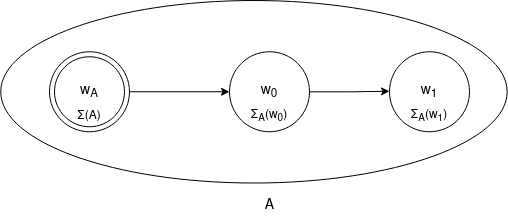
\includegraphics[scale=.5]{Figuras/Modelo.png}
                    \caption[Modelo Etiquetado]{Um exemplo de um modelo etiquetado chamado \(A\), onde \(w_A\) é seu mundo base}
                    \small{Fonte: \me}
                    \label{fig:ModeloEtiquetado}
                \end{figure}

                Considerando, para qualquer mundo \(w_j\) em \Modeloinicial, os conjuntos \(\funcao{S}_{\pi}(\Sigma_{\modeloinicial}(w_j))\)
                de \PI-átomos de \(\Sigma_{\modeloinicial}(w_j)\), esses conjuntos contém todos os elementos (fórmulas pertencentes à \(\Upsilon\)) de fórmulas em \(\Sigma_{\modeloinicial}(w_j)\).
                Estes conjuntos são chamados de \textit{conjuntos de concordância}, pois com base neles construiremos novos \OPImodelos etiquetados
                \Mathcal{N} cujo mundo base é \(w_j\) e que ``concordam'' com a valoração dos elementos dos conjuntos \(\funcao{S}_{\pi}(\Sigma_{\modeloinicial}(w_j))\).

                Para isso, chamaremos o conjunto
                \(\{\varsigma \ | \ \varsigma \in \funcao{S}_{\pi}(\Sigma_{\modeloinicial}(w_j))\} \cup \{\neg \varsigma \ | \ \varsigma \notin \funcao{S}_{\pi}(\Sigma_{\modeloinicial}(w_j))\}\)
                de elementos que são verdadeiros ou cuja negação é verdadeira em \(w_j\), de \textit{diagramas de concordância} e devemos garantir que estes conjuntos são
                \Mathcali{L}{12}-consistentes. Para garantir a consistência destes conjuntos, definimos os conjuntos
                \[
                    \funcao{T}_{\pi}(\Delta) = \{\Box^{n}_{\pi} \delta \ | \ \delta \in \funcao{B}(\funcao{S}_{\pi}(\Delta)) \cap \mathcal{L}_{12} \text{ e } d_\pi(\Box^{n}_{\pi} \delta) \leq d_\pi(\Delta) \}
                \]
                chamados de \PI-teorias e impomos a restrição que \(\funcao{T}_{\pi}(\funcao{S}_{\pi}(\Sigma(\modeloinicial)))\) deve ser verdadeiro em \Mundoinicial. A \PI-teoria
                de um dado conjunto \DDELTA é o conjunto de todos os \(\Box^{n}_{\pi}\text{-fechos}\) de teoremas que são componentes booleanos de fórmulas em \DDELTA, ou seja,
                é o conjunto de todas as fórmulas da forma \(\Box^{n}_{\pi} \phi\), tal que \(\phi\) é um teorema de \(\mathcal{L}_{12}\) e tem forma \(\neg \psi \text{ ou } \psi_0 \lor \psi_1\),
                e \textit{n} é menor ou igual ao comprimento da maior sequência de modalidades \BOXi{\pi} de alguma fórmula no conjunto \DDELTA.
                Como \GAMMA é \Mathcali{L}{12}-consistente e \(\funcao{T}_{\pi}(\funcao{S}_{\pi}(\Sigma(\modeloinicial))) \subseteq \mathcal{L}_{12}\),
                \(\Gamma \cup T_\pi(\funcao{S}_{\pi}(\Sigma(\modeloinicial)))\) é \Mathcali{L}{12}-consistente.
                % Esta é uma operação de seleção de \PI-átomos na definição de \PI-teorias que não é estritamente necessária para
                % provar a transferência de completude, porém permitem provar a transferência de outras propriedades.

                Para cada mundo \(w_j\) no conjunto de mundos de \Modeloinicial, o diagrama de concordância de \(w_j\) é \Mathcali{L}{12}-consistente e está contido em \(\Theta\),
                logo, existe um \OPImodelo etiquetado \Mathcal{N} baseado num frame para \Mathcali{L}{{\overline{\pi}}} que torna este diagrama verdadeiro em algum mundo. Chamaremos de \(w_x\)
                este mundo de \Mathcal{N}, tomaremos ele como o mundo base para \Mathcal{N} e assumimos que este é o único mundo que \Modeloinicial e \Mathcal{N} compartilham.
                O conjunto de elementos de \Mathcal{N} é o conjunto \(\funcao{S}_{\pi}(\Sigma_{\modeloinicial}(w_x))\), que é o conjunto concordância de \(w_x\). Por fim,
                \Mathcal{N} deve tornar a \OPI-teoria de \(\Sigma(\mathcal{N}) = \funcao{T}_{\overline{\pi}}(\funcao{S}_{\overline{\pi}}(\Sigma(\modeloinicial)))\), verdadeira em \(w_{\mathcal{N}}\).

                \begin{figure}[htbp]
                    \centering
                    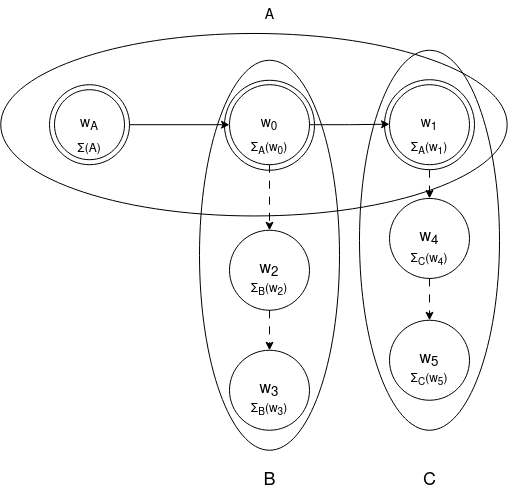
\includegraphics[scale=.5]{Figuras/MultiplosModelos.png}
                    \caption[Modelos Ancorados]{Modelos ancorados em \textit{A}, onde \textit{B} e \textit{C} são do tipo diferente que \textit{A},
                    \(w_0\) é o mundo base de \textit{B} e \(w_1\) é o mundo base de \textit{C}}
                    \small{Fonte: \me}
                    \label{fig:ModelosAncorados}
                \end{figure}

                Caso todas estas condições sejam satisfeitas, \Mathcal{N} é dito \textit{ancorado em} \Modeloinicial no mundo \(w_x\). Ancoramos em \Modeloinicial \OPImodelos etiquetados
                disjuntos (ou seja, que não compartilham mundos entre si) em cada mundo do modelo. Então, cada mundo de \Modeloinicial é o mundo base de algum
                \OPImodelo etiquetado ancorado em \Modeloinicial. Adicionalmente, podemos ancorar \PImodelos etiquetados nos \OPImodelos, ancorados em \Modeloinicial, em mundos que não são base.
                Esta construção pode ser repetida infinitamente. É importante ressaltar que, exceto o modelo etiquetado ancorado em \Mundoinicial em \Modeloinicial,
                nenhum modelo etiquetado será ancorado no mundo base de outro modelo etiquetado. Também é importante ressaltar que modelos etiquetados de um tipo só são ancorados em
                modelos etiquetados de outro tipo, ou seja, \PImodelos etiquetados só são ancorados em \OPImodelos etiquetados, e vice versa.

                Essa relação de ancoramento constrói uma árvore de modelos, onde a raiz é \Modeloinicial e novas folhas são inseridas ancorando modelos em algum modelo folha
                da árvore. Para então avaliar uma fórmula, devemos percorrer a árvore avaliando as subfórmulas da fórmula em modelos compatíveis com a fórmula\footnote{Ou seja, caso
                a fórmula seja do tipo \(\Box_{1}\phi\) ela é avaliada em um 1-modelo e caso a fórmula seja do tipo \(\Box_{2}\phi\) ela é avaliada em um 2-modelo.}.
                Logo, temos uma forma de avaliar, passo a passo, fórmulas que contenham modalidades distintas. Para então construir um 12-modelo que satisfaça o conjunto \GAMMA,
                devemos considerar 1- e 2-modelos ancorados uns nos outros que satisfazem as fórmulas \(\gamma \in \Gamma\). O conjunto de todo conjunto de modelos
                que satisfaz as fórmulas em \GAMMA será chamado de conjunto de \textit{brotos} de \Modeloinicial.

                O lema de Zorn~\cite{zorn1935remark} nos diz que o conjunto de brotos tem um elemento máximo. A união dos elementos (mundos, relações entre mundos e valorações) do elemento
                máximo do conjunto de brotos nos dará o 12-modelo desejado, do qual podemos obter um 12-frame para \Mathcali{L}{12}. Isso quer dizer que, na árvore de modelos gerada
                pela relação de ancoramento, existirá um caminho (sequência de modelos) que satisfaz todas as fórmulas do conjunto \GAMMA, podemos então unir todos os modelos deste caminho
                em um único modelo, do qual podemos obter um frame para \Mathcali{L}{12}.

                \begin{figure}[htbp]
                    \centering
                    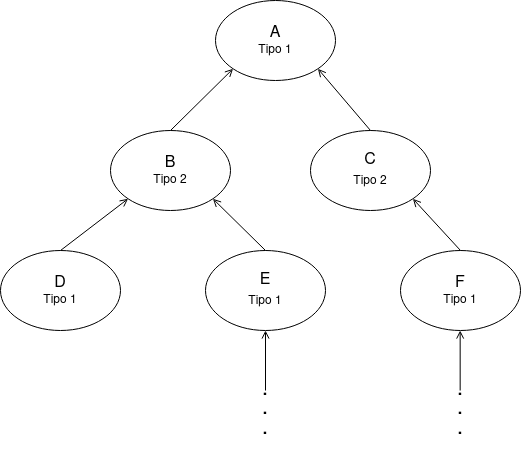
\includegraphics[scale=.5]{Figuras/ArvoreModelos.png}
                    \caption[Árvore de modelos]{Árvore de modelos com raiz em \(A\), onde uma seta indica um ancoramento}
                    \small{Fonte: \me}
                    \label{fig:ArvoreModelos}
                \end{figure}

                Isso conclui a prova informal do Teorema~\ref*{teo:TransCompletude}.
            \end{proof}

            A prova formal do Teorema~\ref{teo:TransCompletude} encontra-se no apêndice~\ref{app:ProvaTransferenciaCompletude}.

            % \begin{exemplo}[Valorando fórmulas em Modelos Ancorados]
            %     ESTE EXEMPLO TALVEZ NÃO ESTEJA CERTO !!!!
            %     Considerando a fórmula \PHI utilizada no Exemplo~\ref{exe:AplicacaoFuncao}:
            %     \[
            %         \phi = \Box_1 (p_0 \lor p_1) \to \Box_2 (p_3 \land (\Box_1 p_0 \lor \Box_2 p_1))
            %     \]
            %     Para valorar \PHI em um mundo \textit{w} de um 1-modelo etiquetado \textit{M}, devemos avaliar as subfórmulas \(\phi_1 = \Box_1 (p_0 \lor p_1)\) e
            %     \(\phi_2 =\Box_2 (p_3 \land (\Box_1 p_0 \lor \Box_2 p_1))\) em \textit{w}. \(\phi_1\) pode ser valorado em \textit{w}, porém \(\phi_2\) deve ser valorado em um 2-modelo
            %     etiquetado \textit{N} ancorado em \textit{M} no mundo \textit{w}. Considerando as subfórmulas \(\phi_3 = \Box_1 p_0\) e \(\phi_4 = \Box_2 p_1\) que devem ser valoradas em \textit{N},
            %     \(\phi_3\) deve ser valorado em um 1-modelo etiquetado \textit{I}, ancorado em \textit{N} em algum mundo \textit{x} tal que \(w \mathcal{R} x\), Já
            %     \(\phi_4\) pode ser valorado em \textit{N}. \qed
            % \end{exemplo}

            \begin{teorema}[Transferência de Completude Forte]
                \label{teo:TransCompletudeForte}
                Sendo \Mathcali{L}{1} e \Mathcali{L}{2} lógicas modais fortemente completas com relação às classes de frames \Mathfraki{F}{1} e \Mathfraki{F}{2},
                então \(\mathcal{L}_{12} = \mathcal{L}_{1} \Odot \mathcal{L}_{2}\) será fortemente completa com relação a classe de frames \(\mathfrak{F}_{12} = \mathfrak{F}_1 \Otimes \mathfrak{F}_2\).
            \end{teorema}

            \begin{proof}[Prova do Teorema~\ref{teo:TransCompletudeForte}]
                Completude forte é exatamente completude generalizada com relação ao espaço de fórmulas \(\mathsf{LM}_{12}\). No enunciado do Teorema~\ref{teo:TransCompletude},
                tome \(\Theta := \mathsf{LM}_{12}\), assim, \(\funcao{DC}_1(\mathsf{LM}_{12}) = \funcao{DC}_2(\mathsf{LM}_{12}) = \mathsf{LM}_{12}\), logo, pelo
                Teorema~\ref{teo:TransCompletude}, provamos o Teorema~\ref{teo:TransCompletudeForte}.
            \end{proof}

            \begin{teorema}[Transferência de Completude Fraca]
                \label{teo:TransCompletudeFraca}
                Sendo \Mathcali{L}{1} e \Mathcali{L}{2} lógicas modais fracamente completas com relação as classes de frames \Mathfraki{F}{1} e \Mathfraki{F}{2},
                \(\mathcal{L}_{12} = \mathcal{L}_{1} \Odot \mathcal{L}_{2}\) será fracamente completa com relação a classe de frames \(\mathfrak{F}_{12} = \mathfrak{F}_1 \Otimes \mathfrak{F}_2\).
            \end{teorema}

            \begin{proof}[Prova do Teorema~\ref{teo:TransCompletudeFraca}]
                Completude fraca é exatamente completude com relação à todo conjunto \(\{\phi\}\) onde \(\phi \in \mathsf{LM}_{12}\). Considerando um \PHI qualquer, no
                enunciado do Teorema~\ref{teo:TransCompletude}, tome \(\Theta = \funcao{B}(\funcao{Sub}(\phi))\). Como o conjunto definido por \(\funcao{Sub}(\phi)\) é finito por
                definição, \(\Theta = \funcao{B}(\funcao{Sub}(\phi))\) contém uma quantidade finita de formulas cujo valor verdade é diferente entre si\footnote{Veja Definição~\ref{def:FuncoesElementos}.}.
                Portanto, existe uma quantidade finita de fórmulas em \(\funcao{DC}_\pi(\Theta)\) que não são equivalente entre si em (um frame/modelo qualquer para) \(\mathcal{L}_\pi\).
                Então, todo subconjunto \(\Delta \subseteq \funcao{DC}_\pi(\Theta)\) é equivalente em (um frame/modelo qualquer para) \(\mathcal{L}_\pi\) a um conjunto de fórmulas finito
                \(\Delta_f\) e, portanto, é equivalente em (um frame/modelo qualquer para) \(\mathcal{L}_\pi\) a uma única fórmula (por exemplo \(\bigwedge \Delta_f\)), que será
                verdadeira no mundo \Mundoinicial no modelo \Modeloinicial, pela Definição~\ref{def:Definicao1}.

                Portanto, \Mathcali{L}{\pi} é completo com relação a \(\funcao{DC}_\pi(\Theta)\), logo, pelo Teorema~\ref{teo:TransCompletude}, \Mathcali{L}{12} é completa
                com relação a \(\Theta\) e, portanto, é completo com relação a \(\{\phi\}\).
            \end{proof}

            Este método de prova é suficientemente genérico para provar a transferência de outras propriedades, sendo necessário apenas pequenas variações em
            em componentes da prova, como demonstrado em~\citeshort{fine1996transfer}.

    \section{O Sistema Bimodal \texorpdfstring{\SisT}{T4}}
        \label{sec:SistemaKT4}
        O sistema bimodal \SisT é talvez um dos sistemas multimodais mais simples, ele consiste da fusão dos sistemas monomodais \textbf{KT} e \textbf{K4}.
        Este sistema será descrito formalmente nesta seção, pois foi usado como estudo de caso para a modelagem de fusão de lógicas modais em Coq, na biblioteca
        descrita no Capítulo~\ref{cap:Implementacao}.

        \subsection{Linguagem, Semântica e Axiomatização}
            \label{subsec:KT4LinguagemSemantica}
            A linguagem \linguagem{\mathcal{T}{4}} do sistema \SisT é baseada na assinatura \({\mathsf{C} = \{\Box_{T}, \Diamond_{T}, \Box_{4}, \Diamond_{4}, \neg, \land, \lor, \to\}}\)
            e é definida abaixo:

            \begin{definicao}[Linguagem de \SisT]
                A linguagem do sistema é \SisT definida indutivamente como o menor conjunto que satisfaz as seguintes regras:
                \begin{align*}
                    & \top, \bot \in \Linguagem{\mathcal{T}{4}}  \\
                    & \mathbb{P} \subseteq \Linguagem{\mathcal{T}{4}} \\
                    & \text{Se } \phi \in \Linguagem{\mathcal{T}{4}} \text{, então } \circ \phi \in \Linguagem{\mathcal{T}{4}}, \circ \in \{\Box_{T}, \Box_{4}, \Diamond_{T}, \Diamond_{4}, \neg\} \\
                    & \text{Se } \phi, \psi \in \Linguagem{\mathcal{T}{4}} \text{, então } \phi \circ \psi \in \Linguagem{\mathcal{T}{4}}, \circ \in \{\land, \lor, \to\} \tag*\qed
                \end{align*}
            \end{definicao}

            \begin{definicao}[\(\mathcal{T}{4}\)-frames e \(\mathcal{T}{4}\)-modelos]
                Um \(\mathcal{T}{4}\)-frame é uma tripla da forma \(\mathcal{F}_{\mathcal{T}{4}} = \langle \mathcal{W}, \mathcal{R}_{\mathcal{T}}, \mathcal{R}_{4} \rangle\),
                onde \(\mathcal{W} \neq \emptyset\), \(\mathcal{R}_{\mathcal{T}}, \mathcal{R}_4 \subseteq \mathcal{W} \times \mathcal{W}\) e \(\mathcal{R}_{\mathcal{T}}\) é uma
                relação reflexiva e \(\mathcal{R}_{4}\) é uma relação transitiva.

                Um \(\mathcal{T}{4}\)-modelo é um par da forma \(\mathcal{M}_{\mathcal{T}{4}} = \langle \mathcal{F}_{\mathcal{T}{4}}, \mathcal{V} \rangle\), onde
                \(\mathcal{V}: \mathbb{P} \to 2^{\mathcal{W}}\) e \(\mathcal{F}_{\mathcal{T}{4}}\) é um \(\mathcal{T}{4}\)-frame. \qed
            \end{definicao}

            \begin{definicao}[Valoração de Fórmulas]
                A valoração de fórmulas em \SisT é definida de forma igual à valoração de fórmulas para lógicas monomodais, com os casos para \BOX e \DIA substituídos por:
                \begin{align*}
                    \mathcal{M}_{\mathcal{T}{4}}, w_0 & \Vdash \Box_{T} \phi \text{ sse } \forall w_1 \in \mathcal{W}, (w_0 \mathcal{R}_{T} w_1 \to
                                    \mathcal{M}_{\mathcal{T}{4}}, w_1 \Vdash \phi)\\
                    \mathcal{M}_{\mathcal{T}{4}}, w_0 & \Vdash \Diamond_{T} \phi \text{ sse } \exists w_1 \in \mathcal{W}, (w_0 \mathcal{R}_{T} w_1 \land
                                    \mathcal{M}_{\mathcal{T}{4}}, w_1 \Vdash \phi)\\
                    \mathcal{M}_{\mathcal{T}{4}}, w_0 & \Vdash \Box_{4} \phi \text{ sse } \forall w_1 \in \mathcal{W}, (w_0 \mathcal{R}_{4} w_1 \to
                                    \mathcal{M}_{\mathcal{T}{4}}, w_1 \Vdash \phi)\\
                    \mathcal{M}_{\mathcal{T}{4}}, w_0 & \Vdash \Diamond_{4} \phi \text{ sse } \exists w_1 \in \mathcal{W}, (w_0 \mathcal{R}_{4} w_1 \land
                                    \mathcal{M}_{\mathcal{T}{4}}, w_1 \Vdash \phi) \tag*\qed
                \end{align*}
            \end{definicao}

            Outros conceitos semânticos são definidos de maneira análoga.

            \begin{definicao}[Axiomatização de \SisT]
                O conjunto de axiomas \(\Lambda_{\mathsf{LM}_{\mathcal{T}{4}}}\) para o sistema \SisT é uma especificação do conjunto \(\Lambda_{\mathsf{LM}_{n}}\) multimodal,
                onde as \textit{n} instâncias do axioma \(K_i\) são substituídas por:
                \begin{align*}
                    & \Box_T (p_0 \to p_1) \to (\Box_T p_0 \to \Box_T p_1) \tag{\(K_T\)} \\
                    & \Box_4 (p_0 \to p_1) \to (\Box_4 p_0 \to \Box_4 p_1) \tag{\(K_4\)}
                \end{align*}
                e com a adição dos axiomas \textit{T}:
                \[
                    \Box_T \phi \rightarrow \phi
                \]
                e \textit{4}:
                \[
                    \Box_4 \phi \to \Box_4 \Box_4 \phi
                \]
                O conjunto de regras de derivação é definido como \(\mathfrak{R} = \{\textit{Nec}_T, \textit{Nec}_4, \textit{MP}\}\).
                Logo, o sistema \SisT pode ser axiomatizada pelo par
                \(\langle\Lambda_{\mathsf{LM}_{\mathcal{T}{4}}}, \{\textit{Nec}_T, \textit{Nec}_4, \textit{MP}\}\rangle\). \qed
            \end{definicao}

        \subsection{Corretude e Completude}
            \label{subsec:KT4CorretudeCompletude}
            Como demonstrado por~\citeauthoronline{blackburn2001modal} (\citeyear{blackburn2001modal}), os sistemas monomodais \textbf{KT} e \textbf{K4} são ambos corretos e fortemente completos, sendo \textbf{KT} correto e fortemente completo
            para a classe \(\mathfrak{F}_{\mathcal{T}}\) de frames reflexivos e sendo \textbf{K4} correto e fortemente completo para a classe \(\mathfrak{F}_{4}\) de frames transitivos.
            Portanto, pelos Teoremas~\ref{teo:TransCorretude} e~\ref{teo:TransCompletudeForte}, temos que o sistema \SisT é correto e fortemente completo para a classe
            \(\mathfrak{F}_{\mathcal{T}4}\) de 2-frames da forma \(\langle \mathcal{W}, \mathcal{R}_{\mathcal{T}}, \mathcal{R}_{4} \rangle\), sendo \(\mathcal{R}_{\mathcal{T}}\) uma relação
            reflexiva e \(\mathcal{R}_{4}\) uma relação transitiva.